\documentclass[runningheads,a4paper]{llncs}

\usepackage{graphicx}
\usepackage{url}

\begin{document}

\mainmatter

\title{Case Study of Using Soft Systems Methodology and UML in a Systems Design Problem in an Agile Environment}
\titlerunning{Case Study of Soft Systems Methodology and UML in an Agile Environment}

\author{James Donohue\inst{1} \and Huseyin Dogan\inst{2}}

\institute{British Broadcasting Corporation, London, United Kingdom\\
\email{james.donohue@bbc.co.uk}
\and
Bournemouth University, Bournemouth, United Kingdom\\
\email{hdogan@bournemouth.ac.uk}}

\maketitle

\begin{abstract}
A generalised software system for the creation and delivery of web syndication feeds, based on the requirements of the British Broadcasting Corporation (BBC) World Service, is considered as a industrial case study in systems design within Agile environments. The design problem is considered first using perspectives from Soft Systems Methodology, leading to the production of a number of UML 2.0 artefacts through the process of analysing and designing the system, incorporating use case and class analysis and sequence and activity diagrams. The authors find that a number of features of SSM and UML remain applicable to information systems design, and reflect on the challenges of using these approaches in organisations such as the BBC that have embraced an Agile approach to software development. Finally suggestions are made for future work to further evaluate and draw connections between theory and current trends in industrial practice.

\keywords{UML, Soft Systems, Agile}
\end{abstract}

\section{Introduction}

The British Broadcasting Corporation (BBC) World Service website portfolio, which currently includes 27 sites but will soon increase to 35, offers news to millions of users around the world in their own language. A publicly-stated ambition of the BBC \cite{bbc2013} is to increase its global audience to 500 million by 2022. One way it can contribute to this effort is through web syndication and the provision of public 'feeds' of its content.

At the time of writing the existing World Service sites are being migrated to a new content management system (CMS) and the `Public Feeds Adaptor' that previously provided web syndication services for these sites is going to be decommissioned. Therefore a new system based around the new CMS must be implemented in order to maintain web syndication capability for the existing 27 sites, and to ensure that it is available for the new ones that will be added.

This paper is an industrial case study of how a large media organisation such as the BBC has put different systems design methodologies into practice in developing a solution to this problem. We consider the relevance of different aspects of the approaches and the challenges of employing them within an industiral context.


\section{Web syndication platform}

Web syndication feeds allows website owners to publish information about new or changed content in a way that can be reused by other websites or end users. Standards for web syndication have existed in some form since 1997 \cite{w3c1997}, the dominant formats today being RSS (Really Simple Syndication) and Atom. Both of these are XML-based and offer a similar feature set, and for the purpose of this study they are treated as equivalent.

Syndication feeds are especially significant to a publisher such as the BBC World Service because such feeds offer an additional channel for distributing news content, circumventing state censorship in countries where the main BBC website may be blocked. RSS and Atom feeds can be easily downloaded and redistributed, and used as a data source for mobile apps, bots and other services. Users of RSS feeds (referred to as 'subscribers') typically use a generic 3rd-party 'reader' application installed on their computer or smartphone, that periodically makes an HTTP request to the BBC's feeds server to retrieve metadata about new and recently updated website content. Such metadata typically includes the titles of news articles and a short description, along with a link to the article itself. In addition to this base level of information, based on editorial policies the BBC may choose to offer 'full text' feeds for certain audiences which include the full article text as well as metadata, in order to facilitate the circumvention described above.

Beyond the well-established RSS and Atom formats, newer formats syndication of web content, often using JSON (JavaScript Object Notation) syntax, are emerging. These formats a range of additional possibilties for sharing news content across different platforms and devices, often with richer and more structured metadata. Although there is no specific requirement to support these formats at present, one requirement for the new syndication platform is to offer greater flexibility around output formats so that they could be added at a later stage.


\section{Methodology}

This study will examine how Soft Systems Methodology (SSM) and the Unified Modeling Language (UML) might be used in the analysis and design of a replacement system for web syndication, and to evaluate the usefulness of these approaches for the current problem. For the purposes of this study, we assume that a new `ideal' system will be built that entirely replaces, and if possible improves upon, the previous one. However, other options are available, such as adapting the legacy system to interoperate with the new CMS. One reason for this assumption is to allow the author freedom to use full range of UML features without being constrained by the existing architecture.

The rationale for the use of SSM and UML together is to determine whether they provide a useful and complementary set of approaches for systems design problems such as the one under examination here. The UML artefacts generated during the investigation will be used as the basis for the iterative design and development of the new system, using an Agile-based development process which is currently the \textit{de facto} standard at the BBC.

Once the system is operational there will be further opportunities to reflect on the relevance of the modelling techniques used by comparing this study with the finished product. In addition, the authors' aim is that the results of this investigation, along with the areas for further research and analysis suggested in the final section, will provide insights as to how organisations such as the BBC might make use of these modelling techniques in future projects.

In the terminology of Soft Systems Methodology (SSM), the starting point for any effort such as this one is a perceived `problematical situation' which is made the subject of a series of learning-focused activities. Checkland and Poulter \cite{checkland2006} see SSM as a shift from the supposed `positivism' of 1950s and 1960s systems engineering methods which sought to solve real-world problems objectively to a phenomenological approach in which the the \textit{Weltanschauung}, or worldview, of all actors is emphasised.


\section{Results}

\subsection{Contextualisation of the problem space through soft systems}

The first Soft Systems activity centres around finding out about the problematical situation. To do this, a \textit{rich picture} may be created as an aide to exploring the context of the problem, and particularly to capture the ``rich moving pageant of relationships'' (\cite{checkland1990}, p.45) between the entities involved.

Fig.~\ref{fig:richpicture} shows shows a rich picture for the present problem. 

\begin{figure}
\centering
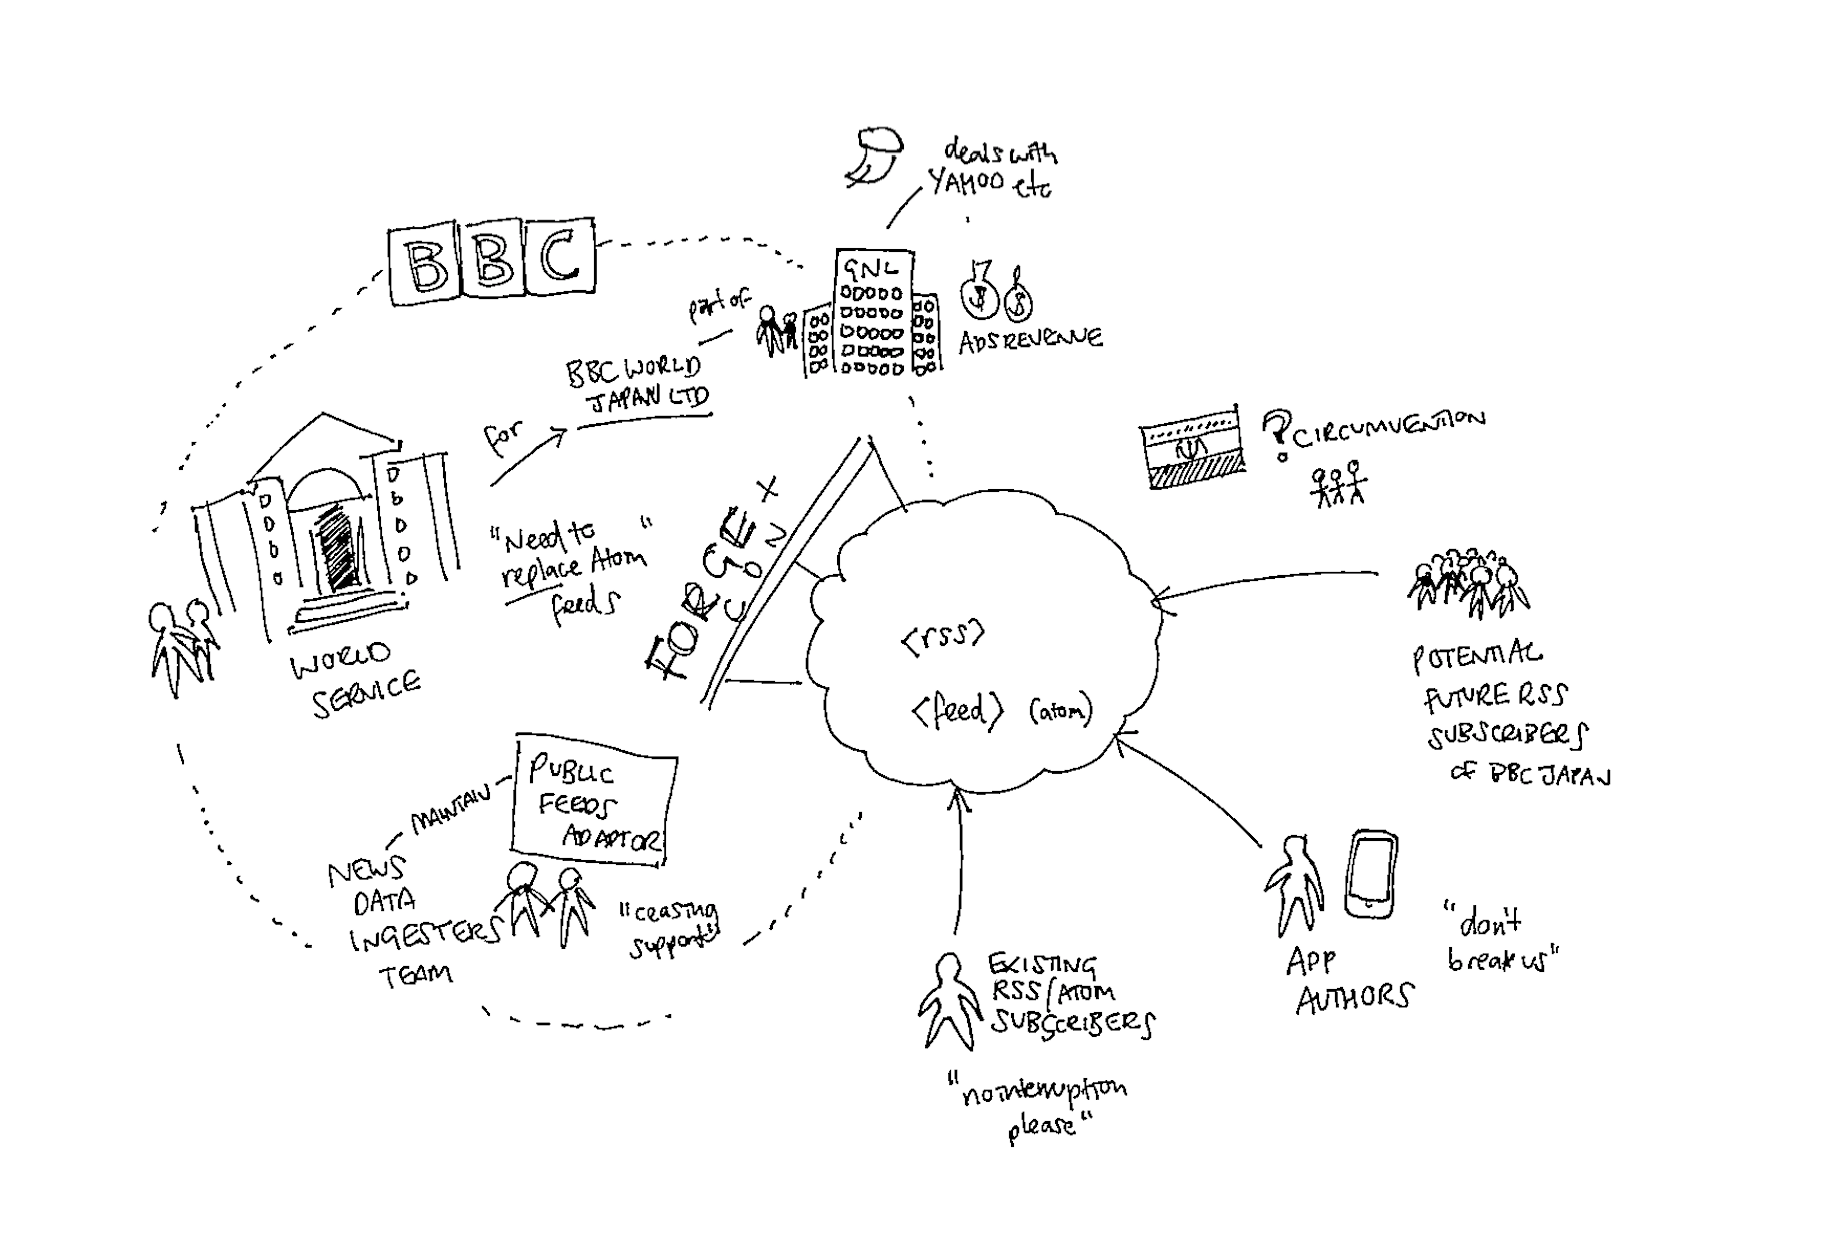
\includegraphics[width=\textwidth]{richpicture}
\caption{Rich Picture of the BBC's problematical situation}
\label{fig:richpicture}
\end{figure}

This rich picture suggests some of the actors whose worldview we should consider. Indeed, SSM's role analysis (known formally as `Analysis One') expands the definition of `issue owner' to be anyone who may be ``concerned about or affected by the situation and the outcome'' (\cite{checkland2006}, p.28). From this perspective, the owners of the issue(s) include the News Product Development Group, the BBC Trust, the Public Feeds Adaptor team and the World Service editorial staff, but also members of the public currently subscribed to feeds, builders of third-party apps that consume the feeds, and even potential future users who do not currently use the feeds.

Next, SSM proposes the creation of a number of models showing `purposeful activity' within a worldview that is made explicit. The starting point for each model is a root definition that describes the system as a statement using the PQR formula (\cite{checkland2006}, p.39). Taking one example from the rich picture, we can write the following root definition:

"A system to provide a new web syndication platform for World Service sites by automatically generating and serving up-to-date RSS feeds, in order to allow users to receive updates about new and changed content and therefore contribute to an increase in website traffic."

As a further step towards enriching our understanding of this system, Soft Systems encourages us to consider the mnemonic CATWOE (\cite{checkland2006}, p.42). Through this we might see a transformation (the T) from a deprecated legacy system with no support for the new CMS, to a better-supported and more flexible platform that will meet the BBC's wider needs in years to come. CATWOE offers a distinction between actors (who are involved in the system's activities), owners and customers who are affected by it. This allows us to refine our list of users given earlier.

Finally, we should give consideration to the environment (the E of CATWOE). There are several dimensions to this, including the operational environment of the BBC itself, but also the context of the changing landscape of web syndication in the age of Twitter and Facebook, with an apparent decline in the importance of feed formats such as RSS. These considerations, and what impact they have on the actors involved, will be touched upon in the use case diagrams and other artefacts produced in the next section.


\subsection{UML artefacts}

In this section we present a series of UML diagrams that explore the problem domain described above. These diagrams are organised according to some of the workflows within the software development lifecycle recommended by the Unified Process (UP).

% UML outputs from section 2


\subsubsection{Use case diagram}

From the root definition and list of actors given earlier, we can create the UML use case diagram shown in Fig.~\ref{fig:use-cases} which is a non-comprehensive depiction of some of the use cases that the system must support. For the purposes of this diagram four actors have been identified, which represent the key roles that users of the system may occupy. The naming of the roles favours typical business usage where this does not agree with modelling guidance. For example the \textsf{Journalist} role could have been named \textsf{ContentEditor} (since the use cases assigned to the role relate to editing content, and this role could be performed by a variety of different individuals not all of whom have the job title \textsf{Journalist}), but this may cause confusion for non-technical stakeholders because of the domain-specific significance of `Editor'. Moreover, as Fowler \cite{fowler2000} (p.43) points out, getting the specific details of actors right is normally less important than finding out the use cases themselves.

\begin{figure}
\centering
\includegraphics[width=\textwidth]{usecases}
\caption{A use case diagram}
\label{fig:use-cases}
\end{figure}

The actor names may be refined, and further roles added, in response to later analysis, since as Arlow and Neustadt \cite{arlow} (p.74), stress, use case modelling is an iterative process. This provisionality applies equally to the system boundary (represented by the black rectangle) that indicates the \textit{subject} of the diagram. For example, for the purposes of illustration we have shown the \textsf{AddContent} and \textsf{UpdateContent} use cases as within the system boundary, but in reality these activities are largely decoupled from the syndication feed management process and could be fulfilled by a separate subject.

One functional requirement of the system is the ability to generate certain defined feeds in a `full text' format which includes the full body text of the article as well as its metadata (title, URL, etc.). This feature is required because some users living in countries with restrictions on Internet access (for example, China) may still be able to access RSS feeds even where access to the originating website has been blocked. Moreover, it creates an opportunity for deliberate circumvention of censorship, since the `full text' feel can be circulated via e-mail, on a USB storage device or even via a custom app, in order to bypass state restrictions on access to international news.

To model this, in Fig.~\ref{fig:use-cases} the \textsf{FulltextSubscriber} actor is a specialised form of the \textsf{Subscriber} actor and therefore a generalisation relationship exists between the two. This entails that \textsf{FulltextSubscriber} inherits all the use cases of \textsf{Subscriber} and adds a third use case, \textsf{GetFulltextFeed}. In order to keep use cases as small and focused as possible, one common area of functionality, \textsf{LogUsage} has been separated out into a separate use case and incorporated via \textsf{<<include>>}. This use use case is more than just an implementation detail: a requirement of the new system identified in discussion with stakeholders is that it should provide more comprehensive logging of requests than the legacy system it replaces, to enable the business to make informed decisions about how to support web syndication in the future (this logging data accessed by the \textsf{CreateUsageReport} use case). We indicate these use cases on the diagram to reflect their relative priority.

In other cases arrowheads have been omitted from actor-use-case relationships as they do not provide significant additional value here (see \cite{ambler}, p.39).

\subsubsection{Use case specification}

In order to describe each use case in more detail, we can use the tabular structure for use case specifications recommended by Arlow and Neustadt \cite{arlow}, an example of which for one of the use cases shown in Fig.~\ref{fig:use-cases} (\textsf{GetFeed}), can be seen in Tab.~\ref{tab:use-case-detail}. In this use case the primary actor (the one who triggers the use case) is the \textsf{Subscriber}. This use case has one major possible alternative flow, which occurs when the subscriber requests a non-existent feed (\textsf{MissingFeed}). An alternative approach would have been to use the \textit{If} and \textit{Else} keywords within the main flow of Table~\ref{tab:use-case-detail} to describe an alternate flow without creating an entire separate specification. This option was rejected on the grounds that it might hinder intelligibility for non-technical readers, since ``use cases are all about communication with the stakeholders'' \cite{arlow} (p.101).

\begin{table}[t]
\begin{center}
\begin{tabular}{ | p{\textwidth} |}
\hline
\multicolumn{1}{|c|}{Use case: GetFeed} \\
\hline
ID: 1 \\
\hline
Brief description: \\
The system return a web syndication feed containing information about content that has recently been created or updated \\
\hline
Primary actors: \\
Subscriber \\
\hline
Secondary actors: \\
None \\
\hline
Preconditions: \\
None \\
\hline
Main flow: \\
1. The use case starts when the Subscriber requests a feed via the network \\
2. The system verifies that there is content for the feed \\
3. The system generates the feed using the options given in the request \\
4. The system returns the generated feed to the Subscriber \\
\hline
Postconditions: \\
None \\
\hline
Alternative flows: \\
GetFeed:MissingFeed \\
\hline
\end{tabular}
\end{center}
\caption{Example of a use case specification}
\label{tab:use-case-detail}
\end{table}


\subsubsection{Analysis model}

The use cases identified in the previous section can be used to produce an analysis model that focuses on \textit{what} the system does (but not yet \textit{how} it does it). Any artefacts produced in this workflow should remain useful to as many stakeholders as possible by using language from the business domain and avoiding implementation details \cite{arlow} (p.122).

The subject of the present study suggests the analysis classes shown in Fig.~\ref{fig:analysis-classes-diagram}. The classes were identified using noun/verb analysis of the project glossary and use cases above, and are named based on clearly identifiable `real world' concepts within the problem domain. They are necessarily high-level at this stage; moreover, features that are typically considerations of design rather than analysis, such as operation parameters, visibility adornments and constructors, have been omitted \cite{arlow} (pp137-8, p148).

\begin{figure}
\centering
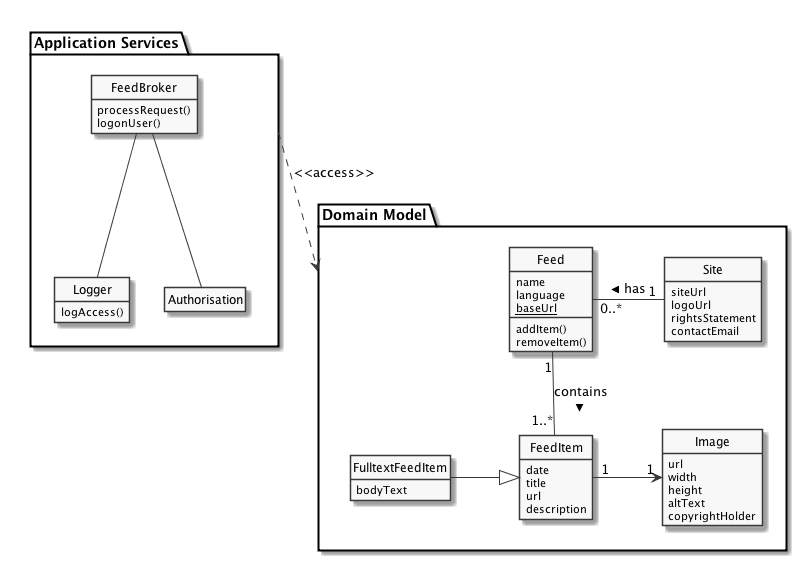
\includegraphics[width=\textwidth]{analysis-classes}
\caption{Analysis classes}
\label{fig:analysis-classes-diagram}
\end{figure}

The contents of the \textsf{Feed} package form the foundations of a \textit{domain model} \cite{fowler2003} for the system that expresses both data and behaviour for the business area, i.e. syndication feeds. However, the only operations shown at this stage within this package (\textsf{addItem()} and \textsf{removeItem()}) are those that may give rise to a state transitions. Also excluded from the diagram are `getter' and `setter' methods for each of the attributes. These methods, which are more properly a feature of design classes, could be represented as pairs of operations for each attribute, e.g. \textsf{getLanguage()} and \textsf{setLanguage()}. Ambler \cite{ambler} considers terms such operations ``scaffolding code'' and points out that they are often automatically generated by modelling tools. Excluding them from class diagrams, as shown here, here may allow readers to more easily see the most significant operations. This also follows Arlow and Neustadt's recommendation to "only show the classes, attributes and operations that illustrate the point you are trying to make" in analysis class diagrams (\cite{arlow}, p.259).

Note that the \textsf{items} attribute of the \textsf{Feed} class is shown with the multiplicity expression \textsf{[0..*]} to indicate that \texttt{null} is a possible value for this attribute, if there are no items. As an alternative to representing class associations diagramatically, we could have shown these relationships using an explicit attribute within the class box (for example, \textsf{items : FeedItem[0..*]}). The diagramatic approach is in our view easier to immediately understand, and avoids having to make assumptions about how associations are implemented during analysis.

To indicate navigability between classes, we have followed \cite{arlow} in suppressing crosses and using a single arrow for unidirectional associations. Following this idiom, it is implicit that the association between \textsf{Feed} and \textsf{Site}, for example, is bidirectional, whereas the association between \textsf{FeedItem} and \textsf{Image} is explicitly one-way. This improves the overall legibility of the diagram, at the expense of some ambiguity.

Although UML supports adding role names at one or both ends of an association to indicate how each class is involved, Ambler (\cite{arlow}, p.65) states that the association name should be sufficient to make roles clear, reserving explicit role names for situations where there are multiple associations between the same classes.

It should be noted that although the analysis model is intended to represent a generic syndication feed, irrespective of any specific serialisation format, it is somewhat aligned to the structure described by the RSS 2.0 Specification\cite{rss}. This is because Atom, the other main competing syndication format, is by and large a functional superset of RSS 2.0, and almost all features of RSS 2.0 can be mapped to an Atom feed without difficulty (for a detailed comparison, see Ruby 2008). Moreover, RSS 2.0 is more widely supported and familiar to developers. For this reason we treat it as a ``lowest common denominator'' of syndication feed formats, while explicitly allowing the system to provide Atom feeds as well.

The \textsf{FulltextFeedItem} represents a specialisation of the generic \textsf{FeedItem} which maps to the capabilities required by the \textsf{GetFulltextFeed} use case described previously. In this situation we have decided to inherit all of the existing data and behaviour of the \textsf{Feed} class and simply add a \textsf{bodyText} member. An alternative approach would be to create an abstract \textsf{GenericFeedItem} class and then provide concrete implementations for both the standard and full-text versions of feed items. However this approach would add greater complexity, and we feel that the risk of coupling \textsf{FulltextFeedItem} to \textsf{FeedItem} is low given there is no requirement to override any of the superclass's operations.

\subsubsection{Use case realisation}

Use case realisation allows us to investigate how analysis classes collaborate in order to bring about the behaviour specified by a use case (\cite{arlow}, p. 241). UML sequence diagrams depict a time-ordered series of interations between instances of different classifiers (here, analysis classes). This allows us to show a dynamic view of some of the static class structure seen in the last section.

Fig.~\ref{fig:sequence-diagram-image} shows a sequence diagram which realises the \textsf{GetFeed} use case seen earlier. This type of diagram is a useful way of communicating the flow of messages between classifiers in a particular situation, in order to give the analyst a better understanding of the roles of each participant and to refine the analysis model further if required. As the left-to-right layout of sequence diagrams can be less familiar to non-techical users than traditional flowchart-style diagrams (see later section on activity diagrams), we have used UML notes to provide a 'script' (organised along the left-hand side of the diagram) to allow the reader to interpret the sequence of events more easily.

\begin{figure}
\centering
\includegraphics[width=\textwidth]{sequence}
\caption{Sequence diagram for \textsf{GetFeed}}
\label{fig:sequence-diagram-image}
\end{figure}

The result of the \texttt{validateFeed} self-delegation message sent by \textsf{FeedBroker} is assigned to a temporary variable, \textsf{isValid}. This enables it to be used in the guard conditions of the \textsf{alt} operator and avoids any repetition of the \texttt{validateFeed} message within the \textsf{alt} section and therefore confusion about how many times it is called. It also reflects a common convention for implementation at the code level.

Note that the \textsf{FeedBroker} object is unnamed (it does not have an identifier before the colon and class name), whereas the specific \textsf{Feed} instance has been given a name (\textsf{mundoFeed}) This follows the recommendation given by Ambler \cite{ambler} (p.86) only to name objects in sequence diagrams when they need to be referenced in messages, the downside being that such a diagram shows a mixture of named and anonymous objects. We feel that during analysis the benefits in terms of reducing diagram clutter outweigh any such disadvantages.


\subsubsection{Design model}

In the design workflow we typically refine the relationships between classes to make them explicit. Fig.~\ref{fig:design-classes-diagram} shows a refinement of some of the design classes from Fig.~\ref{fig:analysis-classes-diagram}. The figure shows only a subset of the domain model classes given in the analysis model in order to focus on one feature, namely the semantics of aggregation relationships.

Attributes and association names have been omitted for clarity, in order to clearly show the semantics of the associations. For example, \textsf{Feed} and \textsf{FeedItem} form a whole-part relationship, and because multiplicity on the `whole' side (\textsf{Feed}) is 1 we can consider this a composition relationship (since a \textsf{FeedItem} may only belong to one \textsf{Feed} and can have no meaningful existence outside of a \textsf{Feed} \cite{arlow} (p.367). Furthermore, feed items share their persistence life cycle with the whole feed \cite{ambler} (p.72). The implication of Fig.~\ref{fig:design-classes-diagram} is that an instance of \textsf{Feed} can navigate to the \textsf{FeedItem}s it contains but not vice versa; if we wanted to allow navigability in the other direction we would have to represent this as an unrefined association arrow in the opposite direction (as seen between \textsf{Feed} and \textsf{Site}) to avoid breaking the asymmetry constraint of aggregation relationships (\cite{arlow}, p.377).

\begin{figure}
\centering
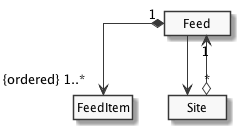
\includegraphics[width=0.5\textwidth]{design-classes}
\caption{Refinement of class relationships during design}
\label{fig:design-classes-diagram}
\end{figure}

Note that we have also added the \textsf{ordered} property to the `part' end of the relationship. This indicates that this one-to-many association must be implemented as an ordered collection of some kind, without placing unnecessary constraints on the implementor by specifying an explicit collection class name. This allows for the most appropriate choice of collection class or type to be used at development time provided it satisfies the constraint (note that \textsf{FeedItem}s are also implicitly unique within the collection - see \cite{arlow}, p.373).

A more thorough development of the design model is beyond the scope of this work, however such an activity would be expected to cover issues such as member visibility and typing of operation parameters and return values. The limited view here is intended to draw attention to just one of the changes in focus that occur when we move from the analysis to the design stage.

\subsubsection{Activity diagram}

After looking at the functionality the system must provide to satisfy use cases, in the design phase we are concerned with the specific details of the system's implementation. Part of this involves ``merging in technical solutions from the solution domain'' (\cite{arlow}, p.333). One architectural constraint that was placed on this project during design was the choice of application technology stack. In order to promote cooperation and resource sharing between different organisational divisions, Morph, a new Node.js application platform developed by BBC Sport, is being used to implement feed generation. Morph has been engineered with a focus on efficiency and provides substantial component-level caching via a data flow model.

\begin{figure}
\centering
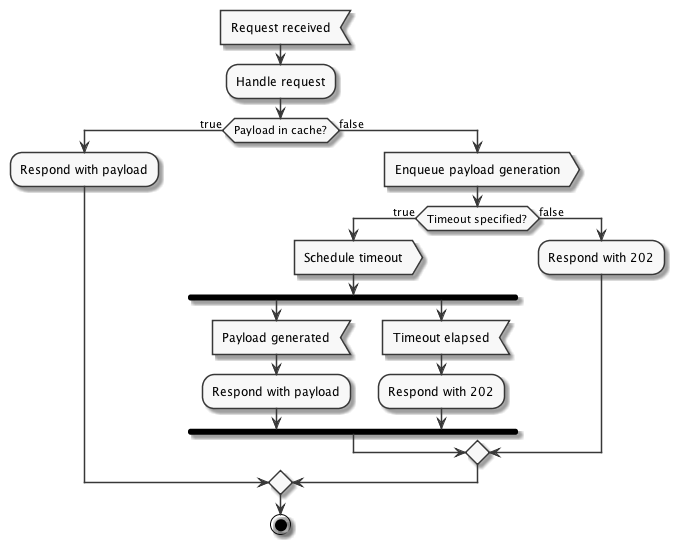
\includegraphics[width=\textwidth]{activity}
\caption{Activity diagram for Morph caching behaviour}
\label{fig:activity-diag}
\end{figure}

Like the majority of dynamic web applications, Morph uses a pull-based model for generating content, the trigger for resource generation being a request made by an HTTP user agent. Once generated, payloads are cached (using Redis, and optionally, Amazon S3). What is different about Morph is that in the event of a cache miss, by default it immediately returns a \texttt{202 Accepted} HTTP response \cite{ietf} to the user, while the request to generate content is queued for asynchronous generation. The semantics of this response are that the client's request was accepted and scheduled for processing (see also \cite{webcaching}).

This corresponds to the `Fail Fast' design pattern proposed by \cite{nygard}, in that the API responds immediately when it determines that it does not have any representation available. One benefit of this approach is that the client can implement a variety of different strategies for retrying and/or recovering, depending on the type of data or functionality being provided.

A UML activity diagram outlining the above approach is give in Fig.~\ref{fig:activity-diag}. This diagram has no explicit initial node, as the \textit{trigger} for this activity is the `accept event' action node (\textsf{Request received}). This node has been placed at the top center of the diagram to make it more natural to read, following Ambler's advice \cite{ambler}, p.115. The signals used in this diagram could be explicitly modelled on a design class diagram using the \textsf{<<signal>>} prototype.

As the diagram indicates, the Fail Fast behaviour described above is modified by the provision of a \texttt{timeout} parameter. This causes Morph to wait for a defined period of time for the response payload to be generated before returning the \texttt{202} response. When this parameter is specified, the outcome depends on which of the two `accept event' actions are triggered first. An alternative way of representing this would be to use an interruptible activity region in conjunction with an `accept time event' action node \cite{arlow} (p.295), but this more esoteric notation has been avoided here in order to make the diagram simpler to understand.


\section{Discussions}

% extract discussions from previous section into here

The figures in this study were generated using PlantUML, a free open-source tool\cite{plantuml} that generates UML artefacts from plain text files.

The UML 2.0 Superstructure specification states that interaction diagrams (of which sequence diagrams are a specialised form) are surrounded by a ``solid-outline rectangle'' including the interaction name in the upper left corner (\cite{omg2011} p.496). Since at the time of writing PlantUML does not support automatically generating this rectangle, it has been manually added before inclusion in this document. Interestingly, PlantUML can produce a `frame' icon that fits the above description when generating deployment diagrams. Since PlantUML is open source software, a helpful contribution to this project (and to the wider UML community) would be to add support for automatically adding the rectangle and title to interaction diagrams in order to make them compliant with the specification. 

Note that frames have not been added to the other diagram types such as class diagrams because they are not mandated by the specification for these types (\cite{omg2011} p.691). This follows the approach taken in the figures in \cite{arlow}.


\section{Conclusions}

This report has included examples of only five of the concrete diagrams in the UML specification, and has only considered the first three workflows of the Unified Process. Further studies could be undertaken to asses the usefulness of other diagram types such as communication diagrams and state machine diagrams in developing similar projects. One particularly rich area for investigation could be the relevance of UML component and deployment diagrams in the light of the recent explosion in Cloud computing and the move away from owned hardware infrastructure and towards Continuous Delivery (CD).

One challenge of using UML for the system being considered here is produced by the technical requirement of the Morph platform being implemented using Node.js. This entails the use of JavaScript as an implementation language. Although JavaScript has matured somewhat since its early days as a web scripting language and is now widely used for back-end systems, it presents some specific challenges since while UML is strongly aligned with the classical inheritance model used by C\# and Java, JavaScript is object-oriented but untyped, (until wider adoption of ECMAScript 6) classless and uses protoypal inheritance. As such, many features of UML class diagrams such as abstract classes and templates are not relevant to JavaScript implementors.

Following on from this, it is important to recognise that while UML offers an effective way of capturing and analysing requirements that describe \textit{what} the system should do, it has limited provision for what are termed ``non-functional requirements''. Constraints on system design such as choice of programming language, but also broader categories such as performance, security and accessibiity do not easily map onto the use case-centric view of systems design shown in UML and must be captured separately (this is considered in Arlow and Neustadt 2005, p.54). It is evident that any user of UML must take special care not to neglect these vital requirements at each stage of the software development life cycle.

It is also worth considering why, given the power of UML both as an analysis tool and as a way of communicating design ideas which we have sought to demonstrate in this study, it is not (at the time of writing) now widely used outside of certain specific industrial contexts. One explanation for the apparent rejection of UML in organisations such as the BBC is the rush since the early 2000s to embrace apparently lower-risk Agile methodologies and UML's association with a now-unfashionable waterfall model of software development. This aversion to `big bang' development has been particularly pronounced in the BBC since the controversy surrounding the overrun and eventual collapse of its Digital Media Initiative project (BBC 2011).

That said, the BBC is by no means alone in this regard. In a recent study (Petre 2013) 70\% of industry respondents said that they did not use UML at all, with most of the remainder saying that they only used it `selectively' (it is worth noting that class, sequence and activity diagrams were among the most used, which supports some of the choices made by this study). One of the main objections cited to UML in the survey was that it focuses too narrowly on architecture and neglects the wider context. This is the antithesis of Checkland's holistic approach to purposeful systems which are always viewed in the context of their environment and the world-view of their users. There is substantial scope for further work on how these two complementary approaches might be usefully combined.


\begin{thebibliography}{}

\bibitem{bbc2013} British Broadcasting Corporation (BBC): BBC announces ambition to double global audience to 500 million,\\
\url{http://www.bbc.co.uk/mediacentre/latestnews/2013/dg-global-audience}

\bibitem{w3c1997} World Wide Web Consortium (W3C): Channel Definition Format (CDF),\\
\url{https://www.w3.org/TR/NOTE-CDFsubmit.html}

\bibitem{checkland2006} Checkland, P., Poulter, J.: Learning for Action: A Short Definitive Account of Soft Systems Methodology and its use for Practitioners, Teachers and Students. John Wiley, Chichester (2006)

\bibitem{checkland1990} Checkland, P., Scholes, J.: Soft Systems Methodology in Action. John Wiley, Chichester (1990)

\bibitem{arlow} Arlow, J., Neustadt, I.: UML 2 and the Unified Process. Second Edition. Addison-Wesley, Upper Saddle River (2005)

\bibitem{ambler} Ambler, S. W.: The Elements of UML 2.0 Style. Cambridge University Press, New York (2005)

\bibitem{fowler2000} Fowler, M., 2000. UML Distilled. Second Edition. Addison-Wesley, Reading (2000)

\bibitem{fowler2003} Fowler, M., 2003. Patterns of Enterprise Application Architecture. Addison-Wesley, Boston (2003)

\bibitem{ietf} Internet Engineering Task Force (IETF): Hypertext Transfer Protocol -- HTTP/1.1,\\
\url{https://www.ietf.org/rfc/rfc2616.txt}

\bibitem{nygard} Nygard, M. T.: Release It!: Design and Deploy Production-Ready Software. The Pragmatic Bookshelf, Raleigh (2007)

\bibitem{omg2011} Object Management Group (OMG): OMG Unified Modeling Language (OMG UML), Superstructure. Version 2.4.1,\\
\url{http://www.omg.org/spec/UML/2.4.1/Superstructure}

\bibitem{petre} Petre, M.: UML in practice. In: 35th International Conference on Software Engineering (ICSE 2013), 18-26 May 2013, San Francisco, CA, USA, pp. 722–731 (2013)

\bibitem{plantuml} PlantUML.com: Frequently Asked Questions\\
\url{http://plantuml.com/faq.html}

\bibitem{rss} RSS Advisory Board: RSS 2.0 Specification. Version 2.0.11,\\
\url{http://www.rssboard.org/rss-specification}

\bibitem{atomrss} Ruby, S.: Rss20AndAtom10Compared,\\
\url{http://www.intertwingly.net/wiki/pie/Rss20AndAtom10Compared}

\bibitem{webcaching} Wessels, D.: Web Caching. O'Reilly, Sebastopol (2001)

\bibitem{bbc2011} British Broadcasting Corporation (BBC): The BBC's management of its Digital Media Initiative,\\
\url{http://downloads.bbc.co.uk/bbctrust/assets/files/pdf/review_report_research/vfm/digital_media_initiative.pdf}

\end{thebibliography}

\end{document}
